\documentclass[serif]{beamer}\usepackage[]{graphicx}\usepackage[]{color}
%% maxwidth is the original width if it is less than linewidth
%% otherwise use linewidth (to make sure the graphics do not exceed the margin)
\makeatletter
\def\maxwidth{ %
  \ifdim\Gin@nat@width>\linewidth
    \linewidth
  \else
    \Gin@nat@width
  \fi
}
\makeatother

\definecolor{fgcolor}{rgb}{0.345, 0.345, 0.345}
\newcommand{\hlnum}[1]{\textcolor[rgb]{0.686,0.059,0.569}{#1}}%
\newcommand{\hlstr}[1]{\textcolor[rgb]{0.192,0.494,0.8}{#1}}%
\newcommand{\hlcom}[1]{\textcolor[rgb]{0.678,0.584,0.686}{\textit{#1}}}%
\newcommand{\hlopt}[1]{\textcolor[rgb]{0,0,0}{#1}}%
\newcommand{\hlstd}[1]{\textcolor[rgb]{0.345,0.345,0.345}{#1}}%
\newcommand{\hlkwa}[1]{\textcolor[rgb]{0.161,0.373,0.58}{\textbf{#1}}}%
\newcommand{\hlkwb}[1]{\textcolor[rgb]{0.69,0.353,0.396}{#1}}%
\newcommand{\hlkwc}[1]{\textcolor[rgb]{0.333,0.667,0.333}{#1}}%
\newcommand{\hlkwd}[1]{\textcolor[rgb]{0.737,0.353,0.396}{\textbf{#1}}}%

\usepackage{framed}
\makeatletter
\newenvironment{kframe}{%
 \def\at@end@of@kframe{}%
 \ifinner\ifhmode%
  \def\at@end@of@kframe{\end{minipage}}%
  \begin{minipage}{\columnwidth}%
 \fi\fi%
 \def\FrameCommand##1{\hskip\@totalleftmargin \hskip-\fboxsep
 \colorbox{shadecolor}{##1}\hskip-\fboxsep
     % There is no \\@totalrightmargin, so:
     \hskip-\linewidth \hskip-\@totalleftmargin \hskip\columnwidth}%
 \MakeFramed {\advance\hsize-\width
   \@totalleftmargin\z@ \linewidth\hsize
   \@setminipage}}%
 {\par\unskip\endMakeFramed%
 \at@end@of@kframe}
\makeatother

\definecolor{shadecolor}{rgb}{.97, .97, .97}
\definecolor{messagecolor}{rgb}{0, 0, 0}
\definecolor{warningcolor}{rgb}{1, 0, 1}
\definecolor{errorcolor}{rgb}{1, 0, 0}
\newenvironment{knitrout}{}{} % an empty environment to be redefined in TeX

\usepackage{alltt}
\usetheme{Boadilla}
\usepackage{graphicx}
\usepackage[final]{animate}
\usepackage{breqn}
\usepackage{xcolor}
\usepackage{booktabs}
\usepackage{tikz}
\usetikzlibrary{decorations.pathreplacing}
\usetikzlibrary{shapes,arrows,positioning,shadows}
\usepackage{subfig}
\usepackage{pgf}

% change format of enumerated lists
\setbeamertemplate{enumerate items}[default]

\setbeamertemplate{navigation symbols}{}

% tikz objects
\tikzstyle{decision} = [diamond, draw, text width=6em, text badly centered, inner sep=2pt, top color=white, bottom color=zissou3]
\tikzstyle{block} = [rectangle, draw, text width=10em, text centered, rounded corners, minimum height=3em, minimum width=8em, top color = white, bottom color=zissou3]
\tikzstyle{declare} = [rectangle, draw, text width=10em, text centered, minimum height=3em, minimum width=8em, top color = white, bottom color=zissou3]

% macros
\newcommand{\emtxt}[1]{\textbf{\textit{#1}}}

% knitr setup


% dependent data


% custom colors
\definecolor{mypal1}{HTML}{EDF8FB}\definecolor{mypal2}{HTML}{B2E2E2}\definecolor{mypal3}{HTML}{66C2A4}\definecolor{mypal4}{HTML}{2CA25F}\definecolor{mypal5}{HTML}{006D2C}

% my custom ggplot theme


\setbeamercolor{title}{fg=mypal5} % main title
\setbeamercolor{frametitle}{fg=mypal4, bg=mypal2} % frame titles
\setbeamercolor{structure}{fg=mypal4} % bottom banner
\setbeamercolor{normal text}{fg=mypal5}
\usebackgroundtemplate{
\includegraphics[height=\paperheight,width=\paperwidth]{fig/back_tmp.pdf}}
\IfFileExists{upquote.sty}{\usepackage{upquote}}{}
\begin{document}

\title[Evaluating water quality]{\textbf{A quantitative and reproducible approach to evaluate trends in seagrass indicators}}
\author[M. Beck]{Dr. Marcus W. Beck}

\institute[USEPA]{ORISE post-doc, USEPA National Health and Environmental Effects Research Laboratory, Gulf Ecology Division, \href{mailto:beck.marcus@epa.gov}{beck.marcus@epa.gov}, Phone: 8509342480}

\date{Dec. 15, 2014}

\titlegraphic{
\centerline{
\begin{tikzpicture}
  \node[drop shadow={shadow xshift=0ex, shadow yshift=0ex}, fill=white,draw] at (0,0) {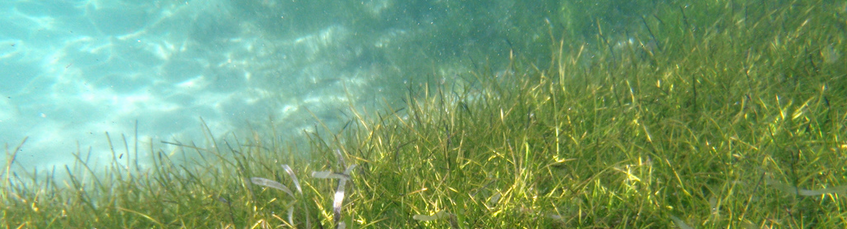
\includegraphics[width=0.8\textwidth]{fig/title_pic.png}};
\end{tikzpicture}
}}

%%%%%%
\begin{frame}[shrink]
\titlepage
\end{frame}

\section{Background}

%%%%%%
\begin{frame}{\textbf{Managing coastal waters}}{\textbf{How do we use data?}}
The foundation of most management programs is a strong monitoring network \\~\\
Monitoring provides information for decision-making based on apparent trends...
\vspace{0.2in}
\begin{center}
\emtxt{What are the changes in environmental condition over time?}\\~\\
\emtxt{Are these changes `good' or `bad' based on our management objectives?}\\~\\
\emtxt{What may have caused these changes?}
\end{center}
\end{frame}

%%%%%%
\begin{frame}{\textbf{Managing coastal waters}}{\textbf{How do we use data?}}
\emtxt{The good news}: We are getting better at monitoring - standardized, automated, increased coverage, real-time/continuous \\~\\
\emtxt{The bad news}: Our ability to use these data for decision-making has not kept pace with availability! \\~\\


{\centering 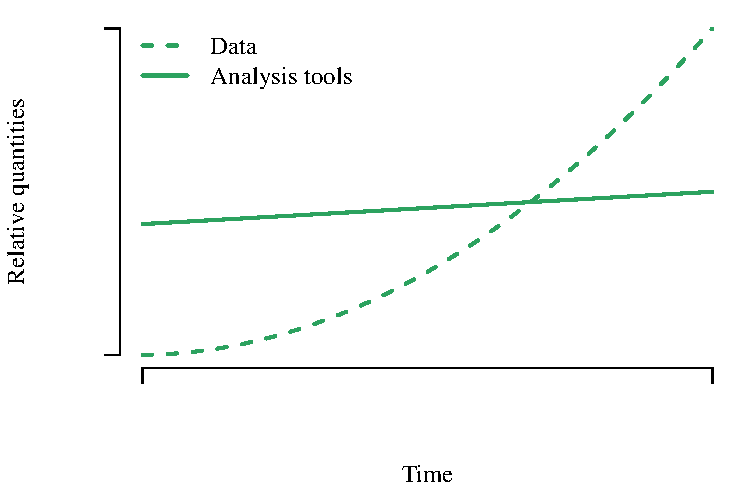
\includegraphics[width=0.55\textwidth]{fig/theo} 

}



\end{frame}

%%%%%%
\begin{frame}{\textbf{Managing coastal waters}}{\textbf{How do we use data?}}
\onslide<+->
We have the data but... \\~\\
\emtxt{Challenge 1:} We may not know how to use the information for decision-making \\~\\
\emtxt{Challenge 2:} We often lack appropriate tools to unambiguously and quantitatively characterize trends \\~\\
\emtxt{Challenge 3:} We may not have indicators to assess progress towards management goals \\~\\
\onslide<+->
These challenges are not impossible...\\~\\
\emtxt{Solution:} The use of open-science tools can facilitate data acquisition, collaboration, and communication!
\end{frame}

%%%%%%
\begin{frame}{\textbf{Seagrasses and water quality}}{\textbf{Making the most of data}}
\onslide<+->
Seagrasses have long been considered sentinels of water quality \\~\\
Numerous ecosystem services - healthy seagrass, healthy eastuary \\~\\
The following example illustrates the use of open-science tools to \emtxt{integrate}, \emtxt{assess}, and \emtxt{communicate} data for evaluating seagrass indicators \\~\\
\onslide<+->
Open-science is \emtxt{reproducible}, \emtxt{transparent}, and \emtxt{collaborative}!
\begin{columns}
\begin{column}{0.2\textwidth}
\centerline{
\includegraphics[width = \textwidth]{fig/Rlogo.png}}
\end{column}
\begin{column}{0.2\textwidth}
\centerline{
\includegraphics[width = \textwidth]{fig/RStudio.png}}
\end{column}
\begin{column}{0.2\textwidth}
\centerline{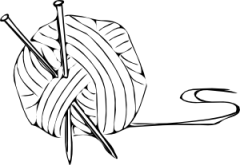
\includegraphics[width = \textwidth]{fig/knit-logo.png}}
\end{column}
\begin{column}{0.2\textwidth}
\centerline{
\includegraphics[width = \textwidth]{fig/octocat.png}}
\end{column}
\end{columns}
\end{frame}

%%%%%%
\begin{frame}{\textbf{Seagrasses and water quality}}{\textbf{Making the most of data}}
\onslide<+->
The maximum depth of colonization is a useful indicator of water clarity - biologically-based and related to numerous response endpoints \\~\\
Often used as a basis for establishing nutrient criteria \\~\\
\onslide<+->
\emtxt{Problem 1:} No consensus on the best way to measure depth of colonization\\~\\
\emtxt{Problem 2:} Plenty of data are available but standardized techniques have not been developed
\end{frame}

%%%%%%
\begin{frame}{\textbf{Seagrasses and water quality}}{\textbf{Making the most of data}}
\onslide<+->
\emtxt{Objective:} Develop a reproducible and empirical method for estimating depth of colonization that leverages multiple data sources
\begin{columns}[T]
\begin{column}{0.5\textwidth}
\begin{knitrout}
\definecolor{shadecolor}{rgb}{0.969, 0.969, 0.969}\color{fgcolor}

{\centering 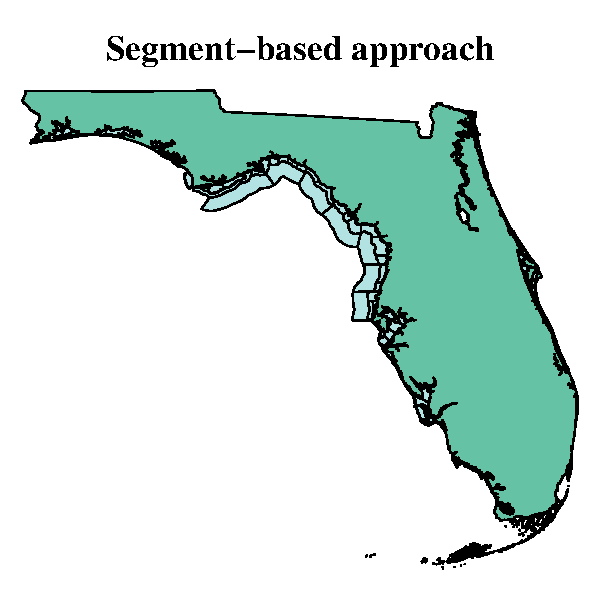
\includegraphics[width=\maxwidth]{fig//segmap} 

}



\end{knitrout}
\end{column}
\begin{column}{0.45\textwidth}
\centerline{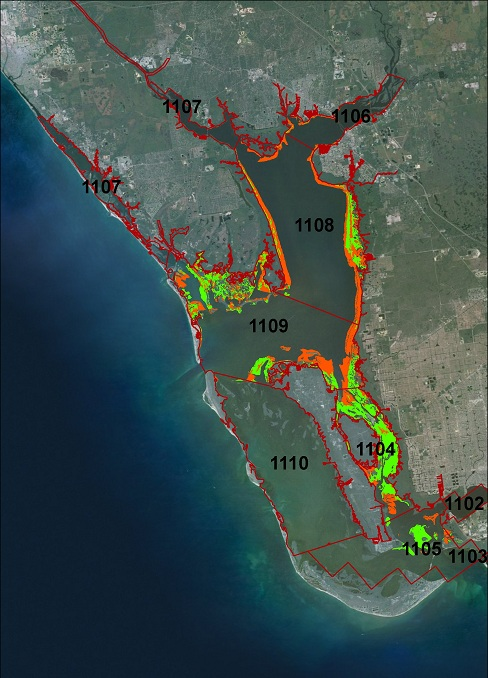
\includegraphics[width = 0.8\textwidth]{fig/Charlotte_Estuary_Segments.jpg}}
\end{column}
\end{columns}
\end{frame}

%%%%%%
\begin{frame}{\textbf{Seagrass and water quality}}{\textbf{Making the most of data}}
\onslide<+->
How can we estimate depth of colonization? \\~\\
\begin{columns}[T]
\onslide<+->
\begin{column}{0.32\textwidth}
Pick a segment\\~\\
\centerline{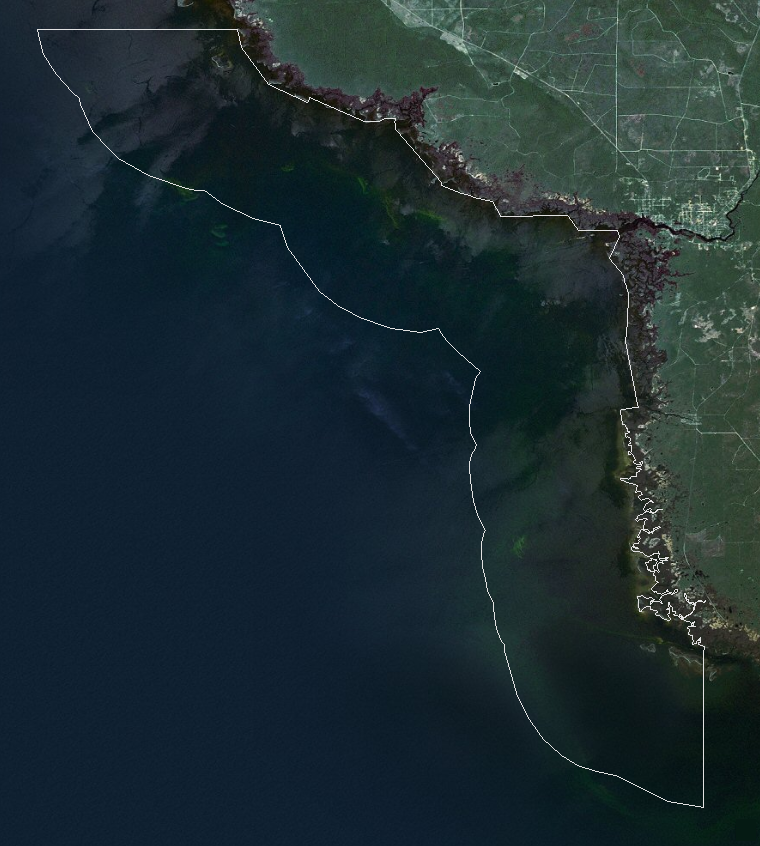
\includegraphics[width = 0.9\textwidth]{fig/map820.png}}
\end{column}
\onslide<+->
\begin{column}{0.32\textwidth}
Get seagrass coverage
\begin{knitrout}
\definecolor{shadecolor}{rgb}{0.969, 0.969, 0.969}\color{fgcolor}

{\centering 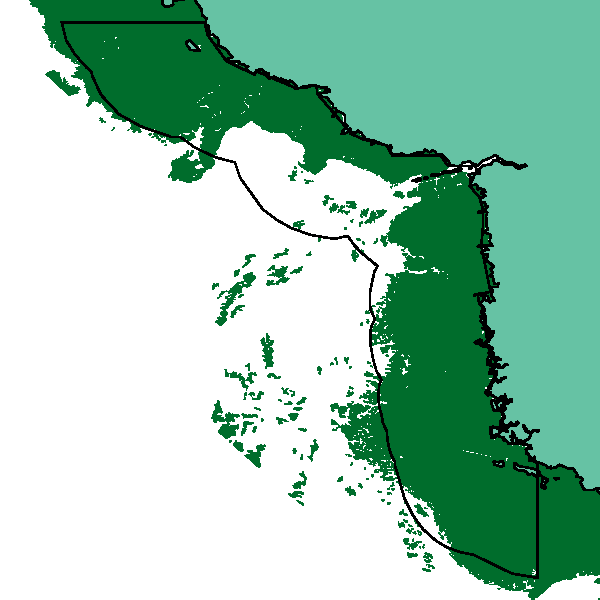
\includegraphics[width=\maxwidth]{fig//segsg} 

}



\end{knitrout}
\end{column}
\onslide<+->
\begin{column}{0.32\textwidth}
Get depth points\\~\\
\begin{knitrout}
\definecolor{shadecolor}{rgb}{0.969, 0.969, 0.969}\color{fgcolor}

{\centering 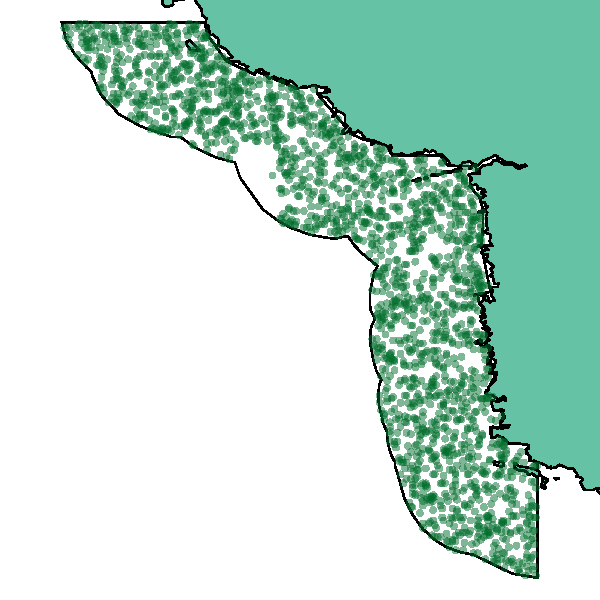
\includegraphics[width=\maxwidth]{fig//segpt} 

}



\end{knitrout}
\end{column}
\end{columns}
\end{frame}

\begin{frame}{\textbf{Seagrass and water quality}}{\textbf{Making the most of data}}
\onslide<+->
How can we estimate depth of colonization? \\~\\


{\centering 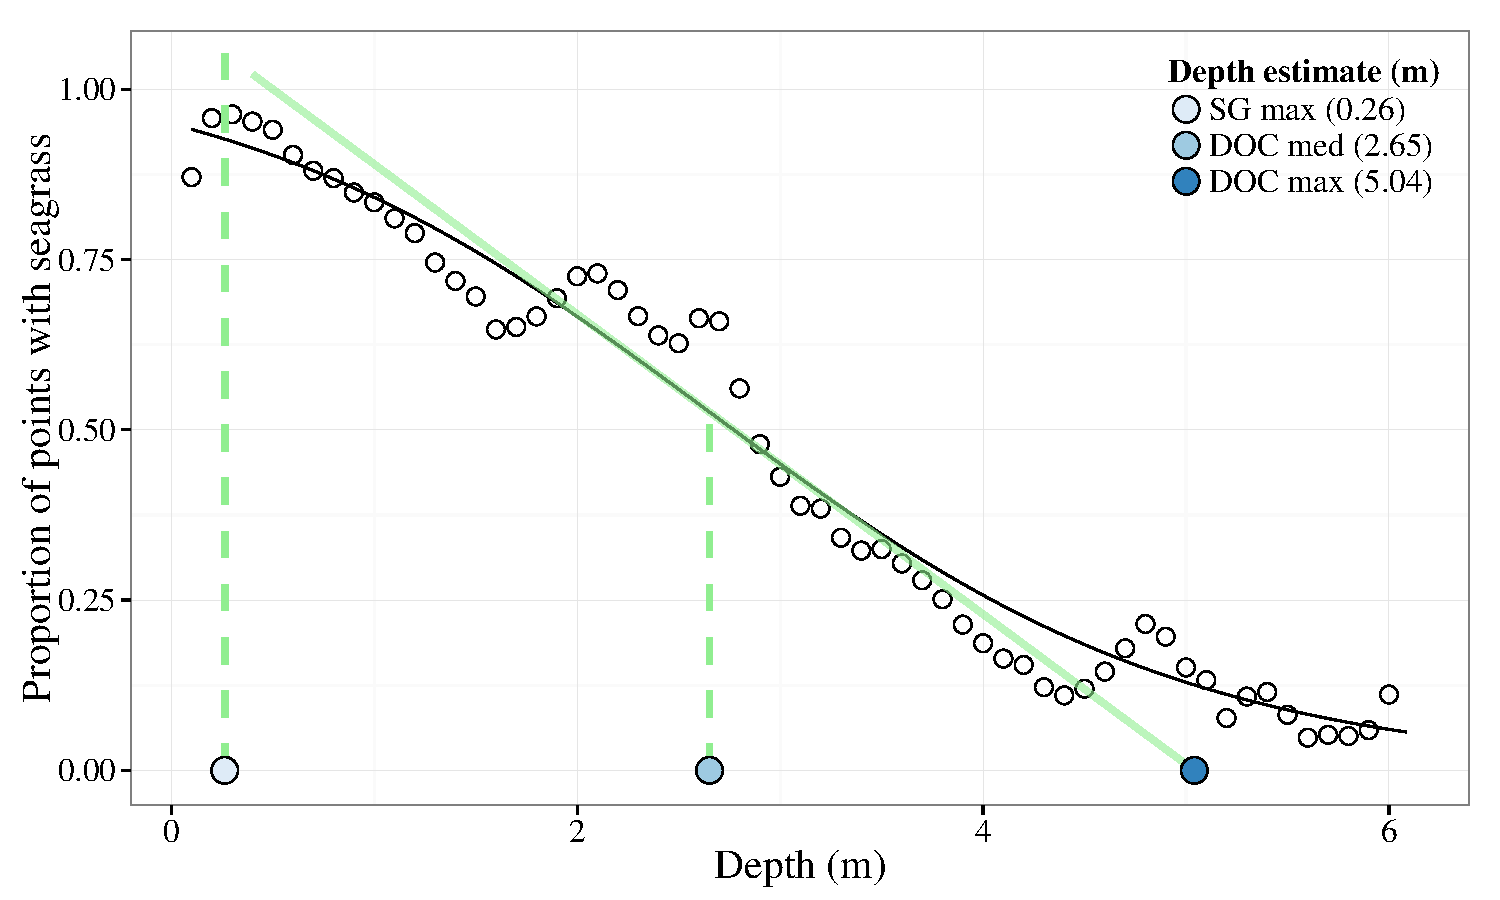
\includegraphics[width=\textwidth]{fig//sg_est_ex} 

}



\end{frame}



%%%%%%
\begin{frame}{\textbf{Seagrass and water quality}}{\textbf{Making the most of data}}
We can get an estimate of seagrass depth of colonization for each segment in Florida \scriptsize [Hagy et al., in prep]
\vspace{-0.25in}
\centerline{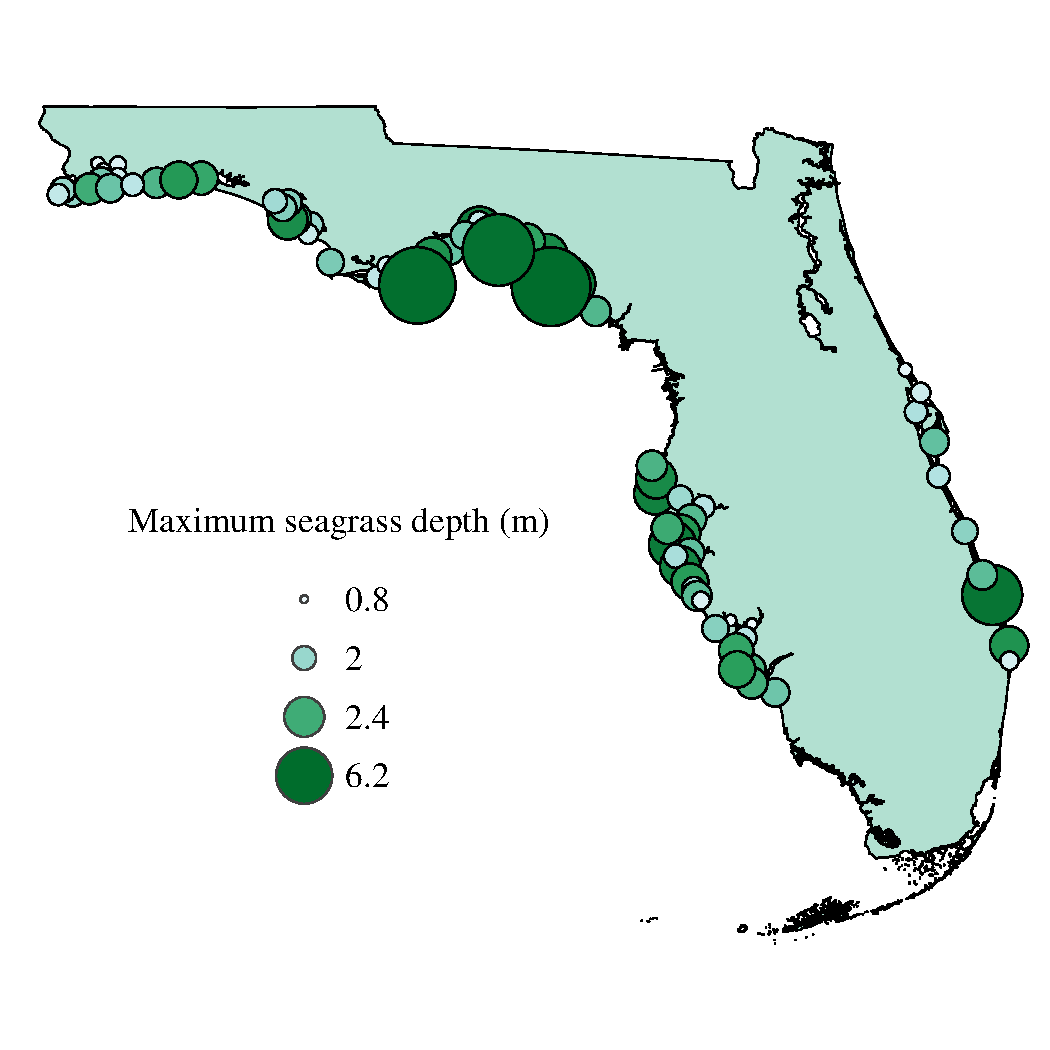
\includegraphics[width = 0.55\textwidth]{fig/sgdepthall.pdf}}
\end{frame}

%%%%%%
\begin{frame}{\textbf{Case 2: Seagrass and water quality}}{\textbf{Making the most of existing data}}
\onslide<+->
This approach works if the segment is an appropriate spatial unit to characterize seagrass...
\begin{columns}[T]
\onslide<+->
\begin{column}{0.45\textwidth}
\begin{knitrout}
\definecolor{shadecolor}{rgb}{0.969, 0.969, 0.969}\color{fgcolor}

{\centering 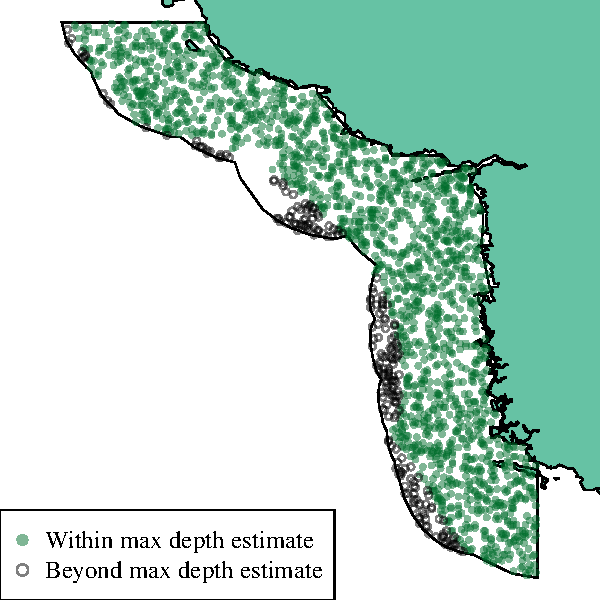
\includegraphics[width=\maxwidth]{fig//docfail1} 

}



\end{knitrout}
\end{column}
\onslide<+->
\begin{column}{0.45\textwidth}
\begin{knitrout}
\definecolor{shadecolor}{rgb}{0.969, 0.969, 0.969}\color{fgcolor}

{\centering 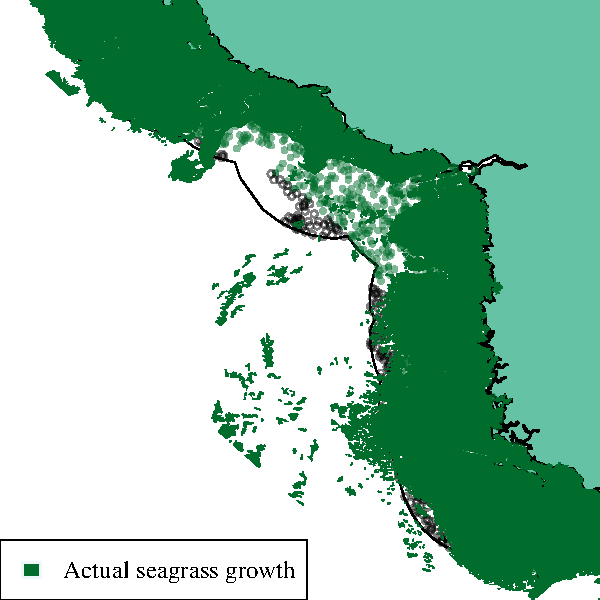
\includegraphics[width=\maxwidth]{fig//docfail2} 

}



\end{knitrout}
\end{column}
\end{columns}
\end{frame}

%%%%%%
\section{References}
\begin{frame}[allowframebreaks,t]{\textbf{References}}
\tiny
\setbeamertemplate{bibliography item}{}
\bibliographystyle{apalike_mine}
\bibliography{ref_diss}
\end{frame}

\end{document}
